% Address the question: What problem are you solving, or opportunity are you seizing? 
\section{1 intro}
Especially in times of a global pandemic, increasing the (psychological) depth of people's remote connections is desirable across the board. Room-scale VR significantly increases the users immersion by, first and foremost, allowing free movements, simulating the sensory \textit{natural} experience in the real world. Further, synchronized motion capture allows avatar movements to be rendered equal to the own bodies movements. In VR, illusions of various kinds (place illusion, plausibility illusion, etc.) occur at the same time for the user to feel present. Depending on the effectiveness of the employed illusions and whether multiple illusions work in congruence, participants experience feeling present in VR \cite{Gonzalez-Franco2017, Kilteni2012}. Most prominently, the embodiment illusion, or body ownership transfer, has proven to elicit \textit{realistic} behavioral as well as physiological responses, when a strong emotional stimulus such as virtual hurting of an embodied rubber hand is provided. Such illusions enrich and/or modify participants subjective experience in VR. Together, free movement, \textit{realisitic} avatar rendering and contextual components of the VR experience coincide at the same time for the user to feel present. Designing immersive experiences for room-scale VR aims at facilitating the emergence of presence experience, dissolving the feeling of connectedness to the real body, ultimately providing the foundation for genuinely connected (social) experiences. 

\section{Zooming in: presence experience and its impact on movement behavior}
In order to scale immersive VR technology to a broader public with use cases ranging from remote office work to entertainment, inclusive design principles are of key importance to successfully designing presence experience across the user base. Individual differences, for example the proclivity to move throughout virtual worlds, significantly challenge designing for presence experience thereby challenging acceptance of VR technology in general \cite{Sagnier2020}. Here, designers and developers would benefit from a rich understanding of user behavior, being able to directly query the impact of certain characteristics of their, unintendedly, neglected user base. Specifically in room-scale VR applications, leveraging inherent motion capture provides the opportunity for data-driven understanding of how individual proclivities explain user experience with spatial specificity. However, typical data reports usually consider aggregate data missing the opportunity to spatially resolve effects of interest.

\begin{figure*}[!ht]
\centering
  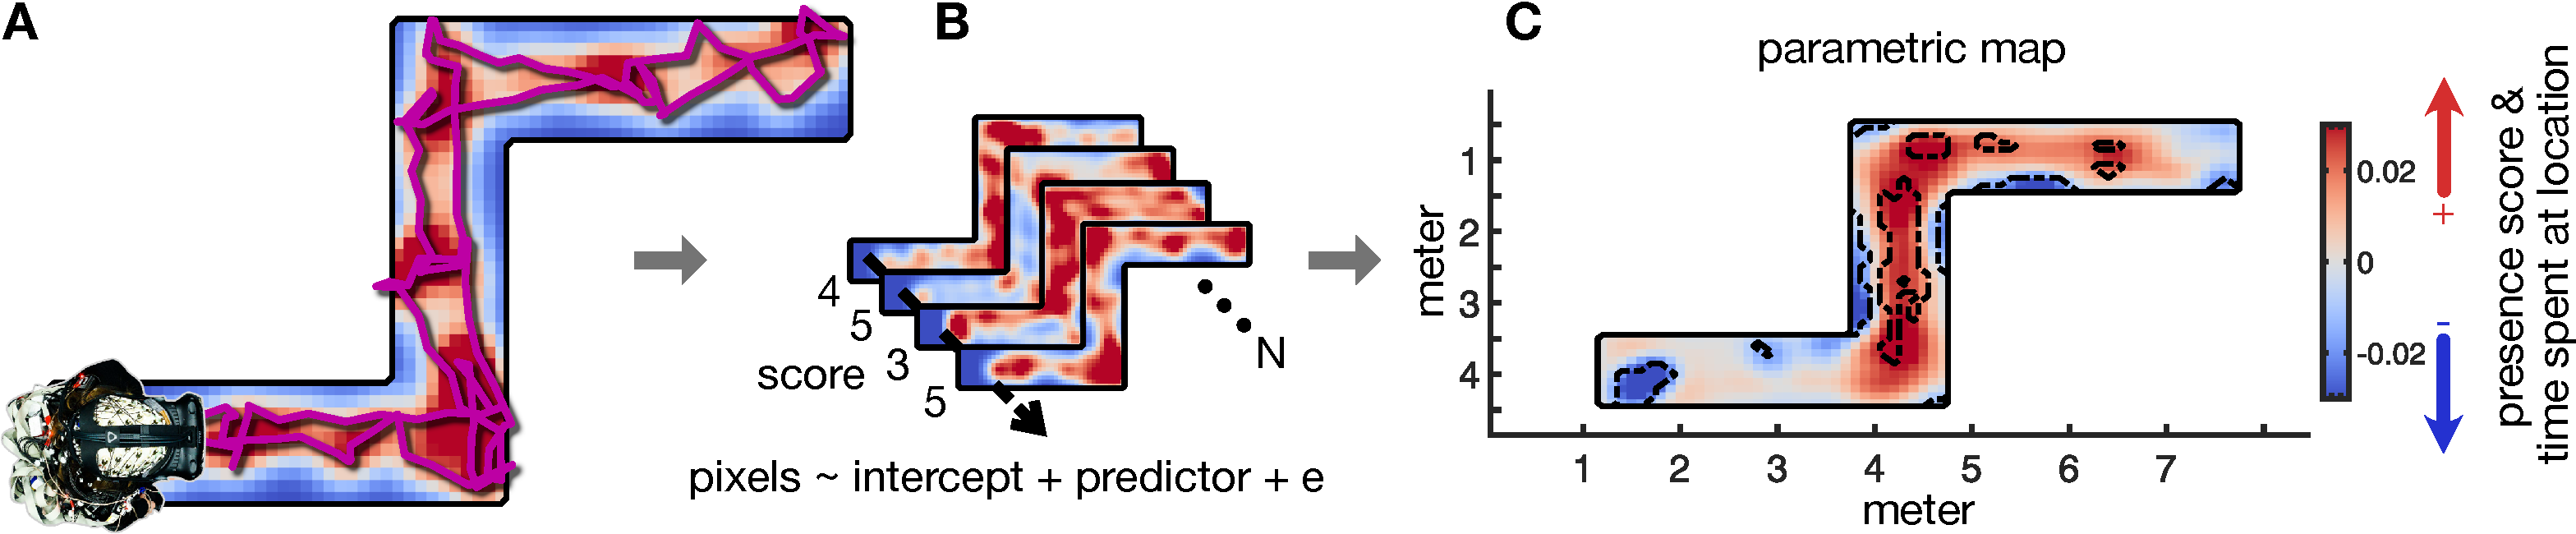
\includegraphics[width=\linewidth]{figures/fig1.pdf}
  %\vspace{-15pt}
  \caption{We propose parametric maps to guide future design decisions of room scale VR applications addressing a broader public. In our study participants explored \textit{invisible} mazes probing hidden walls for visual guidance. \textbf{A:} Motion capture of exploration paths was spatially blurred for across participants analyses of moderating variables. \textbf{B:} We administered experience presence and constructed parametric maps of where participants spent time exploring the mazes as a function of their experienced presence. \textbf{C:} Validating our proposal, we found that with increasing presence, participants were more likely to stay in the center of the paths as well as in segments critical for navigational success.}~\label{fig:methods}
\end{figure*}

We propose using \textit{GLM}, general linear model, in a mass-univariate application across all pixels of a given room-scale VR space. The approach is scalable to many models in the \textit{GLM family} therefore providing a framework with significant flexibility. Further, the analyses scheme is easily extended to 3D space, for example to investigate individual differences in hand reaching scenarios. In this work, we employ the proposed analyses scheme to exhibit how differences in subjectively reported experienced presence impacts participants movement profiles in a \textit{beyond} room-scale VR spatial exploration task. We guide the reader in a step-by-step fashion through the pre-processing, model fitting and inference steps in order to construct spatially resolved \textit{parametric maps}. To highlight potential benefits when considering individual characteristics, we close with a linear regression classification scheme predicting presence via individual characteristics.

%%%%% writing ressources
%As a concurrent effect, we present an easily adaptable and scalable GLM analyses framework to investigate movement behavior with a high spatial resolution.
%Here, we first confirm individual differences in movement profiles of experienced video gamers moving faster and more efficient when exploring a large-scale VR.
